\section{Sintaxis y semántica}

\begin{frame}[fragile]
\frametitle{¿Qué es un programa?}

Un programa es una secuencia de una o mas instrucciones que realizan una tarea en una computadora:

\begin{example}
\begin{semiverbatim}
x = 21;
y = 21;
if (x == y) \{
  z = x + y;
\}
\end{semiverbatim}
\end{example}


\end{frame}

\subsection{Expresiones}

\begin{frame}[fragile]
\frametitle{Sintaxis}
\framesubtitle{Expresiones en Chloe}

\begin{columns}[t]
\column{.45\textwidth}
\begin{semiverbatim}
\textbf{type_synonym} \textit{vname} = string

\textbf{datatype} \textit{exp} = Const \textit{int}
  | Null
  | V      \textit{vname}
  | Plus  \textit{exp} \textit{exp}
  | Subst \textit{exp} \textit{exp}
  | Minus \textit{exp}
  | Div   \textit{exp} \textit{exp}
  | Mod   \textit{exp} \textit{exp}
  | Mult  \textit{exp} \textit{exp}
  | Less  \textit{exp} \textit{exp}
  | Not   \textit{exp}
\end{semiverbatim}
\column{.45\textwidth}
\begin{semiverbatim}
  | And   \textit{exp} \textit{exp}
  | Or    \textit{exp} \textit{exp}
  | Eq    \textit{exp} \textit{exp}
  | New   \textit{exp}
  | Deref \textit{exp}
  | Ref   \textit{lexp}
  | Index \textit{exp} \textit{exp}
and
\textbf{datatype} \textit{lexp} = Deref \textit{exp}
  | Indexl \textit{exp} \textit{exp}
\end{semiverbatim}
\end{columns}


\end{frame}


\begin{frame}[fragile]
\frametitle{Sintaxis}
\framesubtitle{Expresiones en Chloe}

¿Por qué diferenciamos entre \textit{exp} y \textit{lexp}?
\begin{example}
\begin{semiverbatim}
foo = *bar;
*baz = 1;
\end{semiverbatim}
\end{example}



\end{frame}


\begin{frame}[fragile]
\frametitle{Tipos}
\framesubtitle{Enteros y apuntadores}

Los enteros son palabras de precisión 64.
\begin{block}{}
\begin{semiverbatim}
\textbf{type_synonym} int_width = 64
\textbf{type_synonym} int_val = int_width word
\end{semiverbatim}
\end{block}
Y tienen los siguientes límites:
\begin{block}{}
\begin{semiverbatim}
INT_MIN == - (2^(int_width - 1))
INT_MAX ==  ((2^(int_width - 1)) - 1)
\end{semiverbatim}
\end{block}

Un apuntador es un par que representa un identificador de un bloque y un desplazamiento.

\end{frame}


\begin{frame}[fragile]
\frametitle{Memoria dinámica}
\framesubtitle{Diseño del \textit{heap}}

\begin{comment}
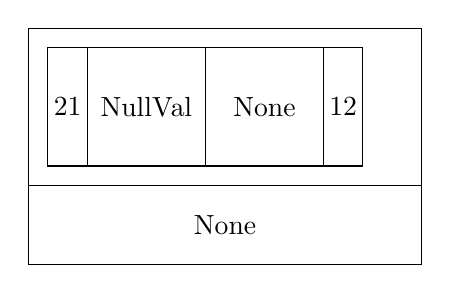
\begin{tikzpicture}
\alert<2>{\draw (0,0) rectangle (5,2); }
\alert<3>{\draw (0,-1) rectangle (5,0) node[midway] {None};}
\alert<4>{\draw (0.25,0.25) rectangle (0.75,1.75) node[midway] {21};}
\draw (0.75,0.25) rectangle (2.25,1.75) node[midway] {NullVal};
\alert<5>{\draw (2.25,0.25) rectangle (3.75,1.75) node[midway] {None};}
\draw (3.75,0.25) rectangle (4.25,1.75) node[midway] {12};
\end{tikzpicture}
\end{comment}


\begin{center}
\begin{tikzpicture}
\alert<2>{\node[draw, minimum width=45mm, minimum height=8mm, label=left:0:] (mem1) {
\begin{tikzpicture}
\alert<4>{\node[draw, minimum width=5mm, minimum height=6mm] (21) {21};}
\alert<4>{\node[draw, minimum width=5mm, minimum height=6mm, right=-\pgflinewidth of 21] (NullVal) {NullVal};}
\alert<5>{\node[draw, minimum width=5mm, minimum height=6mm, right=-\pgflinewidth of NullVal] (None) {None};}
\alert<4>{\node[draw, minimum width=5mm, minimum height=6mm, right=-\pgflinewidth of None] (12) {12};}
\end{tikzpicture}
};}
\alert<3>{\node[draw, minimum width=45mm, minimum height=8mm, below=-\pgflinewidth of mem1, label=left:1:] (mem2) {None};}
\end{tikzpicture}

\bigskip

\begin{itemize}
\alert<2>{\item{Bloque asignado}}
\alert<3>{\item{Bloque Libre}}
\alert<4>{\item{Celdas inicializadas}}
\alert<5>{\item{Celda no inicializada}}
\end{itemize}
\end{center}


\end{frame}


\begin{comment}
\begin{frame}[fragile]
\frametitle{Memoria dinámica}
\framesubtitle{Operaciones de manejo de memoria}

\begin{itemize}
\item<1-3>{new\_block :: $val\ \Rightarrow\ mem\ \Rightarrow\ (val\ \times\ mem)$ option}
\item<1,2,4>{free :: $addr\ \Rightarrow\ visible\_state\ \Rightarrow\ visible\_state$ option}
\item<1,2,5>{load :: $addr\ \Rightarrow\ mem\ \Rightarrow\ val$ option}
\item<1,2,6>{store :: $addr\ \Rightarrow\ val\ \Rightarrow\ visible\_state\ \Rightarrow\ visible\_state$ option}
\end{itemize}

\alert<2>{Los tipos de retorno son $\tau$ option, ya que las funciones siempre pueden fallar.}

\end{frame}
\end{comment}


\begin{frame}[fragile]
\frametitle{Problema de la memoria ilimitada}
\framesubtitle{Soluciones posibles}

La asignación de memoria no puede fallar porque se supone una cantidad ilimitada de memoria.

\bigskip

Sin embargo, se tienen recursos limitados en una computadora.

Hay dos soluciones posibles:

\begin{itemize}
\item{Modelar un comportamiento no-determinístico en la función que asigna memoria.}
\item{Suponer una cantidad fija de memoria.}
\end{itemize}


\end{frame}


\begin{frame}
\frametitle{Problema de la memoria ilimitada}
\framesubtitle{Nuestra solución}

Se mantiene la suposición de memoria ilimitada.

\bigskip
Luego en el proceso de traducción se envuelve la función malloc de C en una definida por nosotros.

\bigskip
Esta función verifica si la llamada a malloc falla.

\bigskip
Si falla, entonces el programa se aborta.


\end{frame}


\begin{frame}
\frametitle{Semántica de las expresiones}
\framesubtitle{¿Cuál es el significado de una expresión?}

La semántica de una expresión es su valor y efecto en el estado del programa.

\pause
\begin{example}
$21 + 21 = 42$

\pause

$foo + 42 = ?$

\pause

$bar = new (12)$
\end{example}
\pause

Se debe saber el valor de una variable a tiempo de ejecución.



\end{frame}


\begin{frame}[fragile]
\frametitle{Semántica de las expresiones}
\framesubtitle{Valuaciones}

Una valuación es una función que mapea un nombre de variable a un valor.

\bigskip
\pause

\textbf{type\_synonym} valuation = vname $\Rightarrow$ val option option

\bigskip

\pause
Dado un nombre de variable puede producir tres resultados diferentes:

\bigskip

\pause
\begin{itemize}
\item{None: valor sin definir.}
\pause
\item{Some None: valor sin inizializar.}
\pause
\item{Some (Some $v$): variable inicializada que tiene valor $v$.}
\end{itemize}


\end{frame}


\begin{frame}
\frametitle{Semántica de las expresiones}
\framesubtitle{Estado visible}

El estado de un programa esta conformado por:
\begin{itemize}
\item Pila de ejecución
\item Variables globales
\item Memoria
\end{itemize}

\pause
Cuando se ejecuta una instrucción, la misma solo puede \textit{ver} cierta parte del estado:

\bigskip
\pause
\begin{itemize}
\item{Variables locales a la función actual}
\pause
\item{Variables globales}
\pause
\item{Memoria}
\end{itemize}


\end{frame}


\begin{frame}
\frametitle{Semántica de las expresiones}
\framesubtitle{Funcioness eval y eval\_l}

Se definen dos funciones para calcular el valor de una expresión.

\bigskip

La evaluación de estas funciones puede fallar:

\bigskip
\pause

\begin{itemize}
\item{Variables sin definir}
\pause
\item{Operandos ilegales dados a la función}
\pause
\item{Acceso a memoria inválida}
\pause
\item{\textit{Overflow} de enteros}
\pause
\item{División por cero}
\end{itemize}


\end{frame}


\begin{frame}
\frametitle{Semántica de las expresiones}
\framesubtitle{Highlights of expression evaluation}
\framesubtitle{Aspectos destacados de la evaluación de expresiones}

\begin{itemize}
\item{Se detecta \textit{overflow} de enteros y lleva a un estado erróneo}
\item{Evaluación de corto circuito}
\item{División y módulo con truncamiento a cero}
\item{Alcance estático de las variables}
\end{itemize}


\end{frame}


\subsection{Instrucciones}


\begin{comment}
\begin{frame}[fragile]
\frametitle{Syntax of commands}
\framesubtitle{Concrete syntax}

\begin{semiverbatim}
com ::= SKIP
     | lexp ::== exp
     | vname ::= exp
     | com ;; com
     | IF exp THEN com ELSE com
     | WHILE exp DO com
     | FREE lexp
     | RETURN exp
     | RETURNV
     | lexp ::== f ( [exp] )
     | vname ::= f ( [exp] )
     | CALL f ( [exp])
\end{semiverbatim}


\end{frame}
\end{comment}


\begin{frame}[fragile]
\frametitle{Sintaxis de las instrucciones}
\framesubtitle{Sintaxis Abstracta}

\begin{semiverbatim}
\textbf{datatype} com = SKIP
             | Assignl lexp exp
             | Assign  vname exp
             | Seq     com  com
             | If      exp com com
             | While   exp com
             | Free    lexp
             | Return exp
             | Returnv
             | Callfunl lexp fname " exp list"
             | Callfun vname fname " exp list"
             | Callfunv fname " exp list"
\end{semiverbatim}

\end{frame}

\begin{frame}[fragile]
\frametitle{Sintaxis de las instrucciones}
\framesubtitle{Llamadas a funciones}

Las funciones no pueden ser expresiones.
\pause

Al llamar a una función hay tres opciones con respecto al valor de retorno:
\pause
\begin{block}{Asignación a celda en memoria}
\verb|Callfunl lexp fname "exp list"|
\end{block}

\pause

\begin{block}{Asignación a una variable}
\verb|Callfun vname fname "exp list"|
\end{block}

\pause

\begin{block}{Asignación sin valor de retorno}
\verb|Callfunv fname "exp list"|
\end{block}


\end{frame}


\begin{frame}[fragile]
\frametitle{Funciones}
\framesubtitle{}

Se tienen funciones que retornan un valor y aquellas que no.

\begin{semiverbatim}
\textbf{record} fun_decl =
  name :: fname
  params :: vname list
  locals :: vname list
  body :: com
\end{semiverbatim}

\bigskip

Una función está bien formada $\Longleftrightarrow$ los parámetros y variables locales tienen nombres diferentes.

\bigskip

Cuando una función retorna un valor, este valor es:

\begin{itemize}
\item{Asignado a una ubicación en memoria}
\item{Asignado a una variable}
\item{Ignorado}
\end{itemize}


\end{frame}


\begin{frame}[fragile]
\frametitle{Programas}

\begin{semiverbatim}
\textbf{record} program =
  name :: fname
  globals :: vname list
  procs :: fun_decl list
\end{semiverbatim}
\pause

\begin{block}{Un programa se considera bien formado si:}
\begin{itemize}
\item{Las variables globales tienen nombres diferentes entre sí.}
\pause
\item{Los nombres de funciones son dieferentes entre sí.}
\pause
\item{Los nombres de variables globales y funciones son diferentes entre sí.}
\pause
\item{Todas las declaraciones de funciones están bien formadas.}
\pause
\item{La función main está definida.}
\pause
\item{Ninguno de los nombres de variables o funciones en el programa es una palabra reservada.}
\end{itemize}
\end{block}


\end{frame}


\begin{frame}[fragile]
\frametitle{Pila de ejecución}
\framesubtitle{Ubicaciones de retorno y marcos de pila}

\textbf{datatype} stack\_frame = com $\times$ valuation $\times$ return\_loc

\bigskip

La pila de ejecución es una lista de marcos de pila.

\onslide<2->{
\begin{semiverbatim}
\textbf{datatype} return\_loc = \alert<3>{Ar \textit{addr}} | \alert<4>{Vr \textit{vname}} | \alert<5>{Invalid}
\end{semiverbatim}

\pause

Un valor de retorno de una función puede ser:
\begin{itemize}
\item<3->{\alert<3>{Asignado a una ubicación en memoria}}
\item<4->{\alert<4>{Asignado a una variable}}
\item<5->{\alert<5>{Ignorado}}
\end{itemize}
}


\bigskip

\end{frame}


\begin{frame}[fragile]
\frametitle{Pila de ejecución}
\framesubtitle{Convención de llamada}

\only<2,4>{
\begin{drawstack}[baseline=(current bounding box.north), scale=0.8]
  \only<2>{
  \startframe
  \cell{x=sum(2,2)}
  \cell{[x$\mapsto$0]}
  \cell{Invalid}
  \finishframe{main}}
  \only<4>{
  \startframe
  \cell{return a+b}
  \cell{[a$\mapsto$2, b$\mapsto$2]}
  \alert<4>{\cell{Invalid}}
  \finishframe{sum}
  \startframe
  \cell{x=sum(2,2)}
  \cell{[x$\mapsto$0]}
  \alert<4>{\cell{x}\only<4>{\cellround{El llamador cambia}}}
  \finishframe{main}
  }
\end{drawstack}
}

\begin{semiverbatim}
\only<1,3>{
int sum(int a; int b){
  return a+b;
}

int main(){
  int x = 0;
  \alert<3>{x = sum(2,2);}
}
}
\end{semiverbatim}


\end{frame}

\subsection{Estados}

\begin{frame}
\frametitle{Tabla de procedimientos y estados}
\framesubtitle{}

La tabla de procedimientos mapea nombres de funciones a sus declaraciones:
\bigskip

\textbf{type\_synonym} proc\_table = fname $\rightharpoonup$ fun\_decl
\pause
\bigskip

Se construye juntando cada declaración de función con su nombre.

\pause
\bigskip

Un estado se define como:
\bigskip
\pause

\textbf{type\_synonym} state = stack\_frame list $\times$ valuation $\times$ mem

\pause

\begin{itemize}
\item{Pila de ejecución}
\item{Variables globales}
\item{Memoria}
\end{itemize}

\end{frame}


\begin{frame}
\frametitle{Estados}
\framesubtitle{Estado inicial}

Un estado inicial es la tupla que contiene:

\begin{itemize}
\item{Pila inicial: Pila de ejecución con el marco de pila de la función main}
\item{Variables globales iniciales: todos los nombres de variables se mapean a indefinido y las varaibles globales a no-inicializado}
\item{Memoria inicial: Memoria vacía}
\end{itemize}


\end{frame}


\subsection{Semántica de pasos cortos}


\begin{frame}[fragile]
\frametitle{Grafo de flujo de control}
\framesubtitle{¿Qué es un CFG?}

Una representación en forma de grafo que cubre los diferentes caminos que un programa puede tomar durante su ejecución.


\begin{figure}
\centering
\tikzstyle{cfg_node} = [circle, draw, fill=uablue25, 
    text width=2em, text centered, minimum height=1em, line width=1pt ]
\tikzstyle{line} = [line width=1pt, -triangle 45]
\tikzstyle{alert} = [text=uared100, fill=uared25, draw=uared100]
\tikzstyle{alert_pp} = [text=uared100]
\tikzstyle{dim} = [text=uablue25, fill=uablue5, draw=uablue25]

\begin{tikzpicture}[node distance=1.5cm, auto]
    % Place nodes
    \node [cfg_node,onslide=<2>{alert}] (c1) {$c_1$};
    \node [cfg_node,onslide=<2>{alert}] (c2) [right of=c1, node distance=3cm] {$c_2$};
    \node [onslide=<6>{alert_pp}](pp) [above left of=c1, node distance=1.5cm] {program pointer};
    % Draw edges
    \draw [line,onslide=<3-5>{alert}] (c1) node[above right of=c1, node distance=1.25cm] {(en, tr)} -> (c2);
    \draw [line,onslide=<6>{alert}] (pp) -> (c1);
\end{tikzpicture}
\end{figure}


\begin{itemize}
\item<2->{Los nodos del CFG son instrucciones}
\item<3->{Las aristas del CFG están anotadas con dos funciones que dependen del estado del programa}
  \begin{itemize}
  \item<4->{La primera indica si una arista puede ser seguida o no}
  \item<5->{La segunda indica como se transforma el estado al seguir una arista}
  \end{itemize}
 \item<6->{Se tiene una ubicación actual, la cual es un \textit{program pointer} al nodo actual}
\end{itemize}


\end{frame}


\begin{frame}
\frametitle{Grafo de flujo de control}
\framesubtitle{Funciones \textit{enabled}}


\begin{figure}[fragile]
\begin{block}{}
\textbf{type\_synonym} enabled = state $\rightharpoonup$ bool
\end{block}

\begin{center}
\begin{tikzpicture}
  [
    grow                    = right,
    sibling distance        = 6em,
    level distance          = 10em,
    edge from parent/.style = {draw, -latex},
    every node/.style       = {font=\footnotesize},
    sloped
  ]
  \node [root] {IF $b$ THEN $c_1$ ELSE $c_2$}
    child { node [env, onslide=<2>{alertnode}] {$c_1$}
      edge from parent node [below, onslide=<2>{alertedge}] {(en\_pos, tr)} }
    child { node [env, onslide=<3>{alertnode}] {$c_2$}
      edge from parent node [above, onslide=<3>{alertedge}] {(en\_neg, tr)} };
\end{tikzpicture}
\end{center}
\end{figure}


\only<1>{Esta función indica si un estado puede continuar su ejecución.

Es una función parcial, por lo que puede fallar.}

\only<2>{Cuando la evaluación de la condición b produce un valor true, se sigue la arista que lleva a $c_1$.}

\only<3>{Cuando la evaluación de la condición b produce un valor false, se sigue la arista que lleva a $c_2$.}

\only<4>{Dependiendo del resultado de la función \textit{enabled} se decide que arista tomar.}

\only<5>{Siempre habrá una arista que pueda ser seguida.}

\end{frame}


\begin{frame}
\frametitle{Grafo de flujo de control}
\framesubtitle{Funciones \textit{transformer}}

\begin{block}{}
\textbf{type\_synonym} transformer = state $\rightharpoonup$ state
\end{block}
\bigskip

Esta función transforma un estado en uno nuevo dependiendo de la arista que se siga.

\bigskip

Es una función parcial, falla cuando se encuentra un error en la transformación.

\bigskip

Esta función actualiza el estado con el estado resultante cada vez que se sigue una arista.



\end{frame}


\begin{comment}
\begin{frame}
\frametitle{Control Flow Graph}
\framesubtitle{How do our transformer functions behave?}

\only<1>{We have a set of functions that will take the neccessary parameters to yield an appropiate transformer function for each command in Chloe.}

\pause
\begin{itemize}
\item\only<2->{{\textbf{tr\_id} :: transformer where tr\_id $\equiv$ Some}}
\item\only<3->{{\textbf{tr\_assign} :: vname $\Rightarrow$ exp $\Rightarrow$ transformer}}
\item\only<4->{{\textbf{tr\_assignl} :: lexp $\Rightarrow$ exp $\Rightarrow$ transformer}}
\item\only<5->{{\textbf{tr\_eval} :: exp $\Rightarrow$ transformer}}
\item\only<6->{{\textbf{tr\_free} :: lexp $\Rightarrow$ transformer}}
\item\only<7->{{\textbf{call\_function} :: proc\_table $\Rightarrow$ fname $\Rightarrow$ exp list $\Rightarrow$ transformer}}
\item\only<8->{{\textbf{tr\_callfunl} :: proc\_table $\Rightarrow$ lexp $\Rightarrow$ fname $\Rightarrow$ exp list $\Rightarrow$ transformer}}
\item\only<9->{{\textbf{tr\_callfun} :: proc\_table $\Rightarrow$ vname $\Rightarrow$ fname $\Rightarrow$ exp list $\Rightarrow$ transformer}}
\item\only<10->{{\textbf{tr\_callfunv} :: proc\_table $\Rightarrow$ fname $\Rightarrow$ exp list $\Rightarrow$ transformer}}
\item\only<11->{{\textbf{tr\_return} :: exp $\Rightarrow$ transformer}}
\item\only<12->{{\textbf{tr\_return\_void} :: transformer}}
\end{itemize}

\end{frame}
\end{comment}


\begin{frame}[fragile]
\frametitle{Grafo de control de flujo}
\framesubtitle{\ldots con una pila.}

\begin{figure}
\centering
\tikzstyle{cfg_node} = [circle, draw, fill=uablue25, 
    text width=1em, text centered, minimum height=1em, line width=1pt ]
\tikzstyle{line} = [line width=1pt, -triangle 45]
\tikzstyle{alert} = [text=uared100, fill=uared25, draw=uared100]
\tikzstyle{alert_pp} = [text=uared100]
\tikzstyle{dim} = [text=uablue25, fill=uablue5, draw=uablue25]
\tikzstyle{dimtext} = [text=uablue25]

\begin{tikzpicture}[node distance=1.5cm, auto, baseline=(current bounding box.north)]
    % Place nodes
    \node [cfg_node] (c1) {$f()$};
    \node [cfg_node] (c2) [right of=c1, node distance=3cm] {$c_2$};
    \node [cfg_node] (c6) [right of=c2, node distance=3cm] {$c_6$};
    \node (pp) [above left of=c1, node distance=1.5cm, onslide=<2->{dimtext}] {program pointer};
    \node (pp3) [above left of=c2, node distance=1.5cm, onslide=<3->{dimtext}] {program pointer};

    \node [cfg_node] (c3) [below of=c1, node distance=3cm] {$c_3$};
    \node (pp2) [above left of=c3, node distance=1.5cm, onslide=<4->{dimtext}] {f()};
    \node [cfg_node] (c4) [right of=c3, node distance=1.5cm] {$c_4$};
    \node [cfg_node] (c5) [right of=c4, node distance=1.5cm] {$c_5$};
    \node (pp4) [above left of=c5, node distance=1.5cm] {};
    % Draw edges
    \draw [line] (c1) -> (c2);
    \draw [line] (c3) -> (c4);
    \draw [line] (c4) -> (c5);
    \draw [line] (c2) -> (c6);
    \draw [line,onslide=<2->{dim}] (pp) -> (c1);
    \draw [line,onslide=<2>{alert}, onslide=<5>{alert},onslide=<3-4>{dim},onslide=<1>{dim}] (pp3) -> (c2);
    \draw [line,onslide=<3>{alert},onslide=<1-2>{dim}, onslide=<4->{dim}] (pp2) -> (c3);
    \draw [line,onslide=<4>{alert},onslide=<1-3>{dim}, onslide=<5->{dim}] (pp4) -> (c5);
\end{tikzpicture}
\end{figure}

\begin{tikzpicture}[stack/.style={rectangle split, rectangle split parts=#1,draw, anchor=center}, baseline=(current bounding box.north)]
\only<2>{
\node[stack=3]{
\nodepart{three}$c_2$
};
}

\only<3>{
\node[stack=3]{
\nodepart{two}$f()$
\nodepart{three}$c_2$
};
}

\only<4>{
\node[stack=3]{
\nodepart{two}$c_5$
\nodepart{three}$c_2$
};
}

\only<5->{
\node[stack=3]{
\nodepart{three}$c_2$
};
}
\end{tikzpicture}


\end{frame}


\begin{frame}[fragile]
\frametitle{Grafo de flujo de control}
\framesubtitle{Reglas}

\textbf{type\_synonym} cfg\_label = enabled $\times$ transformer

\bigskip

\textbf{inductive} cfg :: com $\Rightarrow$ cfg\_label $\Rightarrow$ com $\Rightarrow$ bool

\begin{itemize}
\item{Assign: \textbf{cfg} ($x$ ::= $a$) (en\_always,tr\_assign $x$ $a$) SKIP}
\item{Assignl: \textbf{cfg} ($x$ ::==  $a$) (en\_always,tr\_assignl $x$ $a$) SKIP}
\item{Seq1: \textbf{cfg} (SKIP;; $c_{2}$) (en\_always, tr\_id) $c_{2}$}
\item{Seq2: $[\![$\textbf{cfg} $c_{1}$ $a$ $c_{1}'$ $]\!]$ $\Longrightarrow$ \textbf{cfg} ($c_{1}$;; $c_{2}$) $a$ ($c_{1}'$;; $c_{2}$)}
\item{IfTrue: \textbf{cfg} (IF $b$ THEN $c_{1}$ ELSE $c_{2}$) (en\_pos $b$, tr\_eval $b$) $c_{1}$}
\item{IfFalse: \textbf{cfg} (IF $b$ THEN $c_{1}$ ELSE $c_{2}$) (en\_neg $b$, tr\_eval $b$) $c_{2}$}
\item{While: \textbf{cfg} (WHILE $b$ DO $c$) (en\_always, tr\_id)
  (IF $b$ THEN $c$;; WHILE $b$ DO $c$ ELSE SKIP)}
\item{Free: \textbf{cfg} (FREE $x$) (en\_always, tr\_free $x$) SKIP}
\end{itemize}

\end{frame}


\begin{frame}[fragile]
\frametitle{Grafo de flujo de control}
\framesubtitle{Reglas}

\begin{itemize}
\item{Return: \textbf{cfg} (Return $a$) (en\_always, tr\_return $a$) SKIP}
\item{Returnv: \textbf{cfg} Returnv (en\_always, tr\_return\_void) SKIP}

\item{Callfunl: \textbf{cfg} (Callfunl $e$ $f$ params)
  (en\_always, tr\_callfunl proc\_table $e$ $f$ params) SKIP}
\item{Callfun: \textbf{cfg} (Callfun $x$ $f$ params)
  (en\_always, tr\_callfun proc\_table $x$ $f$ params) SKIP}
\item{Callfunv: \textbf{cfg} (Callfunv $f$ params)
  (en\_always, tr\_callfunv proc\_table $f$ params) SKIP}
\end{itemize}

\end{frame}


\begin{frame}
\frametitle{Semántica de pasos cortos}
\framesubtitle{}

¿Por qué una semántica de pasos cortos?
\bigskip
\pause

Se quiere poder hablar de estados intermedios y diferenciar entre programas que no terminen y programas erróneos.

\bigskip
\pause


\begin{block}{La semántica de pasos cortos se define sobre estados:}
\textbf{inductive} small\_step :: state $\Rightarrow$ state option $\Rightarrow$ bool
\bigskip

$s\ \rightarrow\ s_2$

$\equiv$

``Se toma un paso corto desde $s$ hasta $s_2$''
\end{block}


\end{frame}


\begin{frame}
\frametitle{Semántica de pasos cortos}
\framesubtitle{¿Cuándo se puede dar un paso?}

Un paso desde $s$ hasta $s_2$ se puede dar cuando:
\begin{itemize}
\item{Paso regular:}
\begin{itemize}
\item{Pila no vacía}
\item{Hay una arista en el CFG entre $c_1$ y $c_2$}
\item{La instrucción en el tope de la pila es $c_1$}
\item{Aplicar la función enabled produce True}
\item{Aplicar la función transformer sobre $s$ produce $s_2$}
\end{itemize}
\item{Paso de retorno desde una función sin valor de retorno:}
\begin{itemize}
\item{Pila no vacía}
\item{La instrucción en el tope de la pila es SKIP}
\item{Aplicar la función transformer tr\_return\_void sobre $s$ produce $s_2$}
\end{itemize}
\end{itemize}

\end{frame}


\begin{frame}
\frametitle{Semántica de pasos cortos}
\framesubtitle{¿Cuándo falla el dar un paso?}

Cuando hay una ejecución errónea, se da un paso desde $s$ a None:
\begin{itemize}
\item{Paso regular:}
\begin{itemize}
\item{Pila no vacía}
\item{Hay una arista en el CFG entre $c_1$ y $c_2$}
\item{La instrucción en el tope de la pila es $c_1$}
\item{Aplicar la función enabled o transformer produce None}
\end{itemize}
\item{Paso de retorno desde una función sin valor de retorno:}
\begin{itemize}
\item{Pila no vacía}
\item{La instrucción en el tope de la pila es SKIP}
\item{Aplicar la función transformer tr\_return\_void sobre $s$ produce None}
\end{itemize}
\end{itemize}


\end{frame}


\begin{frame}
\frametitle{Semántica de pasos cortos}
\framesubtitle{¿Cómo dar varios pasos cortos?}

Se lleva la definicón de small\_step a trabajar sobre state option:

\bigskip
\textbf{inductive} small\_step' :: state option $\Rightarrow$ state option $\Rightarrow$ bool
\bigskip
\pause

Para tomar varios pasos se utiliza la clausura reflexivo-transitiva sobre small\_step':

\bigskip
\textbf{inductive} small\_step' :: state option $\Rightarrow$ state option $\Rightarrow$ bool
\bigskip

$s\ \rightarrow*\ s_2$

$\equiv$

``Se toma uno o mas pasos cortos desde $s$ hasta $s_2$''



\end{frame}


\subsection{Interpretador}


\begin{frame}
\frametitle{Interpretador}
\framesubtitle{Ejecución de un programa}

Un paso se ejecuta al aplicar la función \textit{transformer} correspondiente al estado y actualizar la instrucción en el tope de la pila.
\bigskip
\pause

La semántica es determinística, lo que permite escribir un interpretador para la misma.
\bigskip
\pause

\begin{block}{Interpretar un programa:}
Mientras no se alcance un estado final, se ejecuta un paso.
\end{block}

\pause

\begin{block}{Ejecutar un programa:}
Verificar que el programa está bien formado.

Si lo es, se interpreta.
\end{block}

\bigskip

El interpretador retorna un estado final o None, que indica una ejecución errónea.

\end{frame}

\begin{frame}[fragile]
\frametitle{Correctitud}
\Fontvi

Se demuestran varias propiedades con respecto a la semántica y el interpretador con asistencia de Isabelle/HOL.

Tomemos como ejemplo la prueba del siguiente teorema:



\begin{columns}[t]
\column{.45\textwidth}
\begin{semiverbatim}
lemma cfg_has_enabled_action:
  assumes " c \\notequal SKIP"
  shows "\\exists c' en tr. cfg c (en,tr) c'
    \\and (en s = None \\or en s = Some True)" 
  using assms
proof (induction c)
  case (Seq c1 c2)
  show ?case
  proof (cases "c1 = SKIP")
    case True
    thus ?thesis by (auto intro: cfg.intros)
  next
    case False
    from Seq.IH(1)[OF this]
      show ?thesis by (auto intro: cfg.intros)
  qed
next
\end{semiverbatim}
\column{.45\textwidth}
\begin{semiverbatim}
  case (If b c1 c2)
  show ?case
  proof (cases "en_pos b s")
    case None[simp]
    thus ?thesis
      by (fastforce intro: cfg.intros)
  next
    case (Some a)[simp]
      show ?thesis
      proof (cases a)
        case True
        thus ?thesis
          by (fastforce intro: cfg.intros)
      next
        case False[simp]
        have "en_pos b s = Some False" by simp
        hence "en_neg b s = Some True"
          unfolding en_pos_def en_neg_def
          by (auto split: Option.bind_splits)
        thus ?thesis
          by (fastforce intro: cfg.intros)
      qed
  qed
qed (auto intro: cfg.intros)
\end{semiverbatim}

\end{columns}


\end{frame}

\begin{frame}
\frametitle{Correctitud}

Se demuestran dos principales teoremas.

\begin{theorem}[La semántica es determinística]
$s \rightarrow s' \land s \rightarrow s'' \Longrightarrow s' = s''$

$s \rightarrow' s' \land s \rightarrow' s'' \Longrightarrow s' = s''$
\end{theorem}

Para demostrar estos dos lemas fue necesario demostrar 9 lemas previos.


\begin{theorem}[El interpretador es correcto con respecto a la semántica]
$\mathtt{terminates}\ cs\ \Longrightarrow\ \mathtt{yields}\ cs\ cs'\ \longleftrightarrow\ (cs'\ =\ \mathtt{interp}\ \mathtt{proc\_table}\ cs)$
\end{theorem}

Para demostrar este lema fue necesario demostrar 6 lemas previos.

\end{frame}

